\chapter{Background}
Rather than assume you are familiar with the various concepts or leave you to trawl external sources this chapter aims to provide sufficient background about fundamental aspects needed to understand the domain / context of the research. Some of the concepts and terms I use in the rest of my thesis are also explained here.

\section{Conceptual Model of Apps and App Stores}
This section introduces a conceptual model of apps and app stores and presents four views of apps in an app store together with various implications of the views, relationships and interactions. 

The research is situated in apps that are available in app stores. App stores house millions of apps and serve billions of users. They also present a rich tapestry of perspectives on software apps and the ecosystem. There has been a great deal of research that focus on particular areas of these apps and sometimes connect these areas as part of the research. My research focuses on an area seldom investigated, namely it focuses on the developer's view of how their app is perceived by the app store.

\begin{figure}[ht]
    \centering
    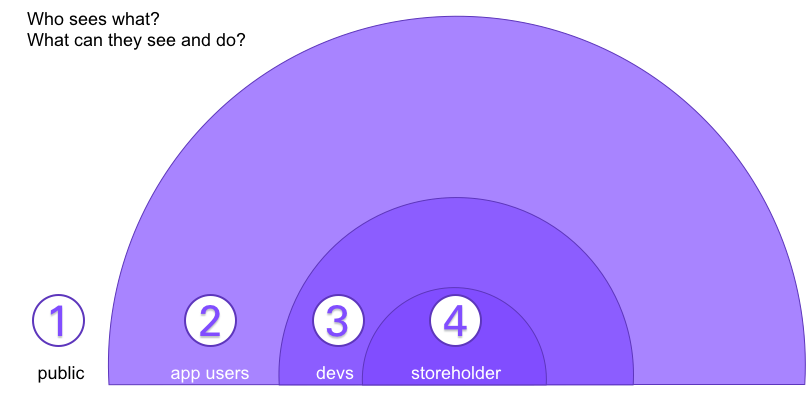
\includegraphics[width=12cm]{images/who-sees-what.png}
    \caption{Four Views of an App Store}
    \label{fig:4-views-of-apps-in-app-store}
\end{figure}

Figure~\ref{fig:4-views-of-apps-in-app-store} illustrates the four views; broadly, those closer to the centre can see what those in outer rings can see. 

The first view is the public view of the app store, what is visible to someone who is not actively engaged with the app store. Examples include people who are not logged into their account, search engines, researchers mining the app store for ratings and reviews, and so on. The public is able to see aggregate ratings and some recent reviews for specific apps. Older reviews are generally hidden from public view (which may limit some research and search engine insights).

The next view is that of a user of a particular app or set of apps. They may have installed some of the apps directly, they are likely to also have pre-installed apps on their device too. They have the ability to interact with the app store, for instance they can see, create, and update their ratings and reviews~\footnote{If supported by the app store, for instance Google Play does.}. They can also see the public view.

Developers have the next view, which includes information the app store records about their interactions with the app store, and information the app store provides the developers directly (\emph{i.e.} generated by the app store and related entities), as well as feedback provided by users via the app store (\emph{e.g.} ratings and reviews). Developers can also see the public view, they cannot see the entire view of their user-base, however they can see any rating and reviews provided by the users.

Both the users and the developers can often see individual ratings and reviews for much longer periods than presented in the public view. Importantly, their primary communications goes via the app store, rather than being direct, and aspects of these communications are often public for a period. The communications and implications will be covered later in this section.

The final view is that of the app store, the `storeholder' in the figure. They have a global and holistic view of the entire store, including potentially all the reviews, user interactions, and whatever usage activities have been performed by all the other three views.

We now cover various implications of the app store conceptual model.

\subsection{Trust relationships}
One of the key success factors of the modern app store (typified by the Apple App Store and Google Play) was the platform provider provided the entire ecosystem and established the rules of engagement. The locus of trust is the provider of the app store acts as the public face and to some extent also acts as a representative for both the users and the developers. In terms of financial transactions it also acts as the intermediary and facilitates users being able to obtain refunds for app and in-app purchases subject to various conditions. 

Note: There are many details related to the trust relationships for those interested in that topic, however in the interests of focus and concision they are outside the scope of this thesis. 

\subsection{Communications paths and data flows}
There are numerous communication paths for mobile apps both with and without an app store being involved. As the vast majority of apps and users use devices and apps that are part of an app store ecosystem (even if they are obtained from other sources, e.g. as often occurs in India) I will only consider the ecosystem that includes an app store in this thesis. Figure~\ref{fig:sources-of-info-with-app-store-background-ch} illustrates various sources of information for apps available in an app store. The sources and communications paths will be considered next. 
% SHOULD-DO Perhaps a Venn diagram would also complement this illustration?

\begin{figure}[ht]
    \centering
    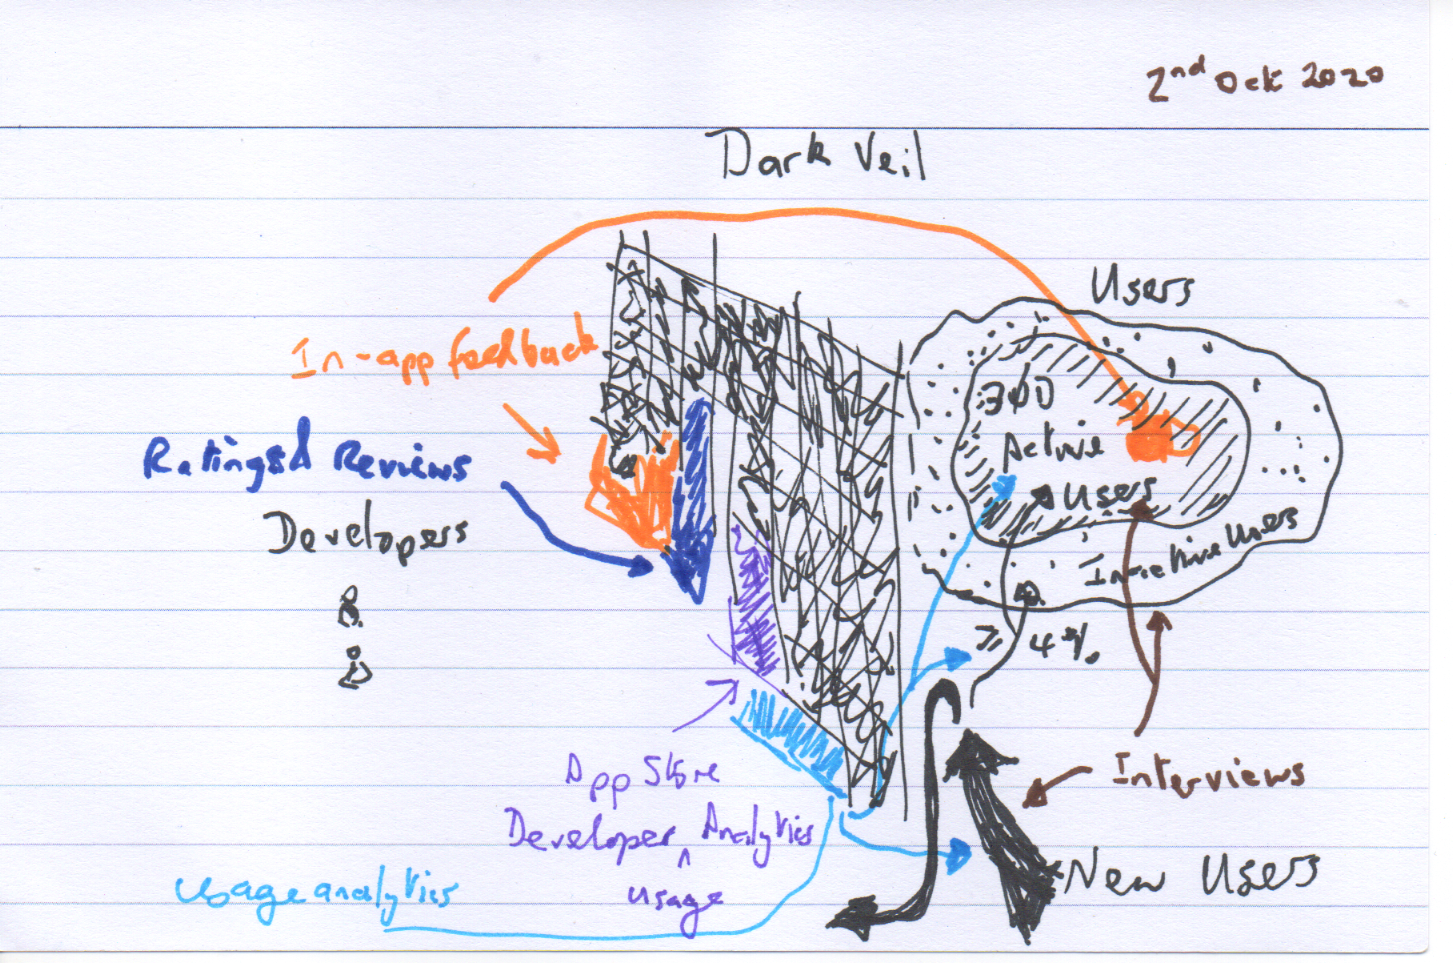
\includegraphics[width=13cm]{images/rough-sketches/sources-of-information-with-app-store-1.png}
    \caption{Sources of information with an App Store}
    \label{fig:sources-of-info-with-app-store-background-ch}
\end{figure}

The information about mobile apps can come from users directly or indirectly, from the app if it collects information either directly or indirectly, from devices (via the operating system, installed apps with privileges to access information about other apps, from accessibility services, and potentially other means e.g. installed viruses), from intermediaries - particularly the app store, and also from network traffic, observers,~\emph{etc.} 

Source code and source code repositories are also useful sources of information about mobile apps. Information can be usefully combined from several sources, for instance from source code about calls to write log messages compared to actual logs recorded when the app has been used on a device. Given the app store plays a pivotal role let's consider its role in terms of communication paths now. 

An app store is more than the store front, it controls and affects many aspects of the ecosystem that gathers around it. It is also more than the software, data and information that the various memberships can access. For instance the modern app stores often include software that is mandatory and pre-installed on end-user devices where that software cannot be easily removed or disabled by users\footnote{competent, technically savvy individuals may be able to thwart protection mechanisms as may other specialist organisations and software.} . This software includes a local storefront that offers end-users new apps, updates, and enables users to manage optional apps\footnote{Optional apps can be installed and uninstalled by end users at will. Non-optional apps are installed by various organisations, including the app store provider, some device manufacturers, and so on.}.

The app store provides various primary communications paths between the various parties involved in the ecosystem. It may be an active party, for instance in some of the reports provided to developers and/or users, and in policy-related matters; or it manages communications between app users and developers. Often the app store's owners define the rules of communications, including details such as whether and when apps can ask users to rate an app.

\begin{figure}[ht]
    \centering
    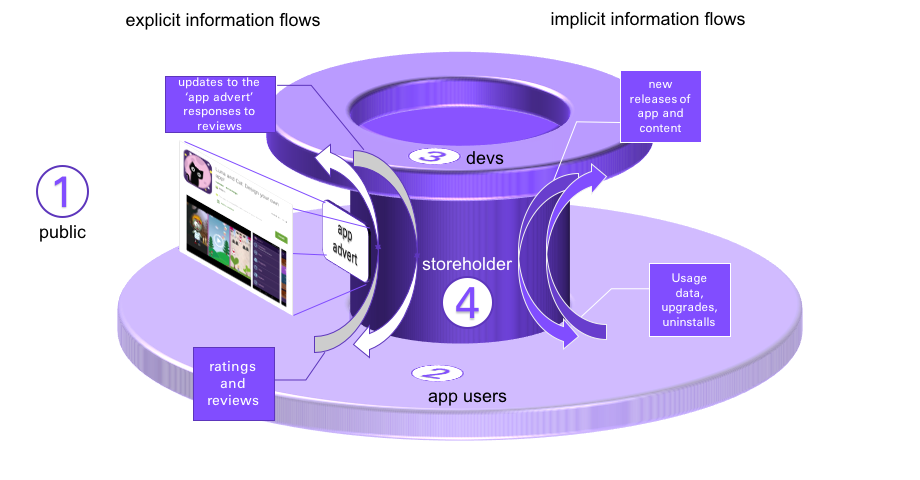
\includegraphics[width=17cm]{images/app-store-data-flows-3d.png}
    \caption{App Store: Communications Paths and Data Flows}
    \label{fig:app-store-data-flows}
\end{figure}

Some of the communications involves humans, or pseudo-humans such as bots. Other communications is generated by software, for instance usage and diagnostic data collected by the operating system and related utilities on a mobile device (collectively described as the platform).

The communications paths and data flows in an app store ecosystem are illustrated in Figure~\ref{fig:app-store-data-flows}. There are two forms of data flows: explicit and implicit. Explicit data flows are actively and intentionally performed by one or more of the participants, implicit data flows represents information that can be inferred or gleaned from various actions and inactions.

Examples of explicit actions intended to communicate include:
\begin{itemize}
    \item Making the app available in the app store; this includes creating screenshots, a description of the app, adding meta data the app store requires and/or requests, \emph{etc.} This information becomes public if the app store approves the app for release.
    \item Ratings and reviews performed by app users. Only a subset of users provide these, the percentage varies from zero to a maximum of around 10\% with typical percentages around 1\% to 3\%. % SHOULD-DO find credible source for these estimates, I've checked various sources without success
    Estimates vary, partly as the definitions vary too. AppBrain states 46.5\% of Android apps do not have a rating~\footnote{Their definition is \emph{``Apps that have less than 3 ratings we consider to not have a rating yet"}~\url{https://www.appbrain.com/stats/android-app-ratings}}. In comparison, 42matters.com estimate 41\% of Android apps and 57\% of iOS apps have no rating~\footnote{\url{https://42matters.com/stats}}.
    \item Google Play, for example, allows developers to respond to reviews, and for both reviewers and developers to update their reviews and responses.
\end{itemize}
%%%%%%% Various interesting sources of Android- (and some iOS) related stats
% https://www.businessofapps.com/data/app-statistics/
% https://www.statista.com/statistics/266217/customer-ratings-of-android-applications/ (seems to be a rehash of AppBrain's report)
% https://mindsea.com/app-stats/
% 


Implicit information flows include:
\begin{itemize}
    \item New releases of apps and related content (such as in-app content, often purchased using in-app purchasing). These indicate the developer is wishes to actively engage their userbase. Upgrades may include changes to the app seeded by various sources such as ratings and reviews and other data, including:
    \item Usage data and upgrades, both imply the software provides some value to the users. Lack of usage may also be an indication the software is not currently providing value - this may be expected for instance with seasonal apps. Uninstalls are a stronger signal that users no longer see sufficient value in the app to keep it on their device.
\end{itemize}

On-device bug reports may be a hybrid, where the bug reporting utility on the device does much of the data collection and may report this automatically and transparently, however it may sometimes ask the user for additional input and permission to send the bug report.

\subsection{Membership criteria of each group}
%\akb{Explain why the membership criteria are important to understand, perhaps combine with next section single explanation of groups and what members can do in each}
As Figure~\ref{fig:app-store-data-flows} illustrates there are four numbered groups in the illustration. People can potentially belong to more than one group (albeit membership of the storeholders is limited to owners and those they assign membership to,~\emph{e.g.} as administrators of the app store). Group membership constrains what the members can do as participants and what they have access to.

\begin{enumerate}
    \item Public: the membership criteria are minimal. Here `public' is any entity, human or technological, that has access to the app store\footnote{For our purposes we can assume online digital access, other modes may also be viable, for instance some researchers use archives of data sourced from app stores.}. An example of a technological entity, is a search engine crawler or software including web scraper technology and scripts that use APIs provided to obtain information about apps in the app store.
    %\akb{Not sure what is meant by 'minimal' here. You could describe 'public' as any entity, human or technological, that has access to the app store. Provide an example of a technological entity, e.g., a search engine crawler}
    \item App user: the public can use an existing account or create a new account with the app store that would allow them to become an app user~\footnote{They need to meet the criteria of the app store.}. Note: there may be restrictions or constraints that mean not everyone can install every app on every device, however the general practice is that apps are freely available for app store users to install on any device they possess. 
    \item Developer: developers need to be registered and validated by the app store, the process varies for specific app stores, they often involve payment of a fee and some amount of validating their identity. Some app stores may perform additional checks based on information they and/or others hold.  
    \item Storeholder: they are generally a legal entity, and certainly for the purposes of this research they are. Apart from a few exceptions (such as F-Droid~\footnote{Details are available online at~\url{https://www.f-droid.org/en/about/}}) they are multi-national major corporations, and again for my research they are.
\end{enumerate}


\subsection{What participants can and cannot do (and who dictates the rules?)}
%\akb{You don't explain the link between the implicit/explicit data flows and these membership groups.}
\begin{itemize}
    \item Public: The public cannot review an app or easily download the app. They can view publicly accessible information, including information that was gathered previously, potentially by others.
    \item App user: They can rate and review apps they have installed on their account~\footnote{ user may have several devices and choose not to install an app on all of them. Also some apps may by limited to devices that meet particular criteria e.g. the platform version.} or device. They can also install, update and deinstall apps~\footnote{There may be restrictions imposed for some apps, for instance Google Apps and Manufacturer apps might be blocked from being uninstalled, and updates are sometimes mandatory, \emph{etc.}}.
    \item Developer:  Approved developers can upload apps to the app store and publish them if the app store also approves the release. They can choose to submit new versions of their apps, sometimes they may be required to do so by the app store. They can choose to suspend or withdraw their app from the store, note: generally users can continue to use the app if they have it installed. Developers are expected to interact with the app store and often do so of their own volition, for instance to see how their app is `doing'. The developer may define a price for their app and/or any in-app purchases. They may also require users comply with additional terms of use, and many apps do so.
    \item Storeholder: They are by far the most powerful participant as they establish the ecosystem including the rules of engagement and enforce these rules. The app store has the right of delay or veto of releases, it can suspend apps and developers, and much else besides. They are expected to comply with the laws of the various countries the app store is available in and also where their business is situated. These laws may affect the developers and the app users, for instance the amount of sales tax charged on a purchase in the app store.
\end{itemize}

We have already identified four membership groups involved in app store ecosystems, there is at least one more and also additional data flows in the ecosystem. The fifth membership group is a~\emph{service provider}. These service providers provide non-trivial functionality and other capabilities such as in-app analytics, feedback, and so on. Developers can choose to incorporate software libraries into their apps and use the services provided, for instance as conduits of communications between the app and the developers. Here developers include other specialist groups in their organisation such as customer service personnel and marketing teams. Many app developers choose to use at least one such service, some incorporate several and there is even specialist software that enables developers to manage multiple similar services within their apps on end-user devices. An example of this type of software is~\url{https://github.com/segmentio/analytics-android} (other platforms are also supported and there are other providers of similar software).

Membership matters in particular because of who has access to which data and for how long they have access. Note: Control and `ownership' of the data are also relevant topics, however they are not necessary to comprehend the rest of this topic. % SHOULD-DO consider whether to add material on this topic in the thesis. 

\section{Three layers of an app}
In some of my earlier work, published in ~\citep{harty_aymer_playbook_2016}, I introduced the concept of three layers of an app. These are illustrated in Figure \ref{fig:3-layers} and shows three primary conceptual layers related to a mobile app.

\begin{figure}[ht]
    \begin{minipage}{\textwidth}
    \centering
    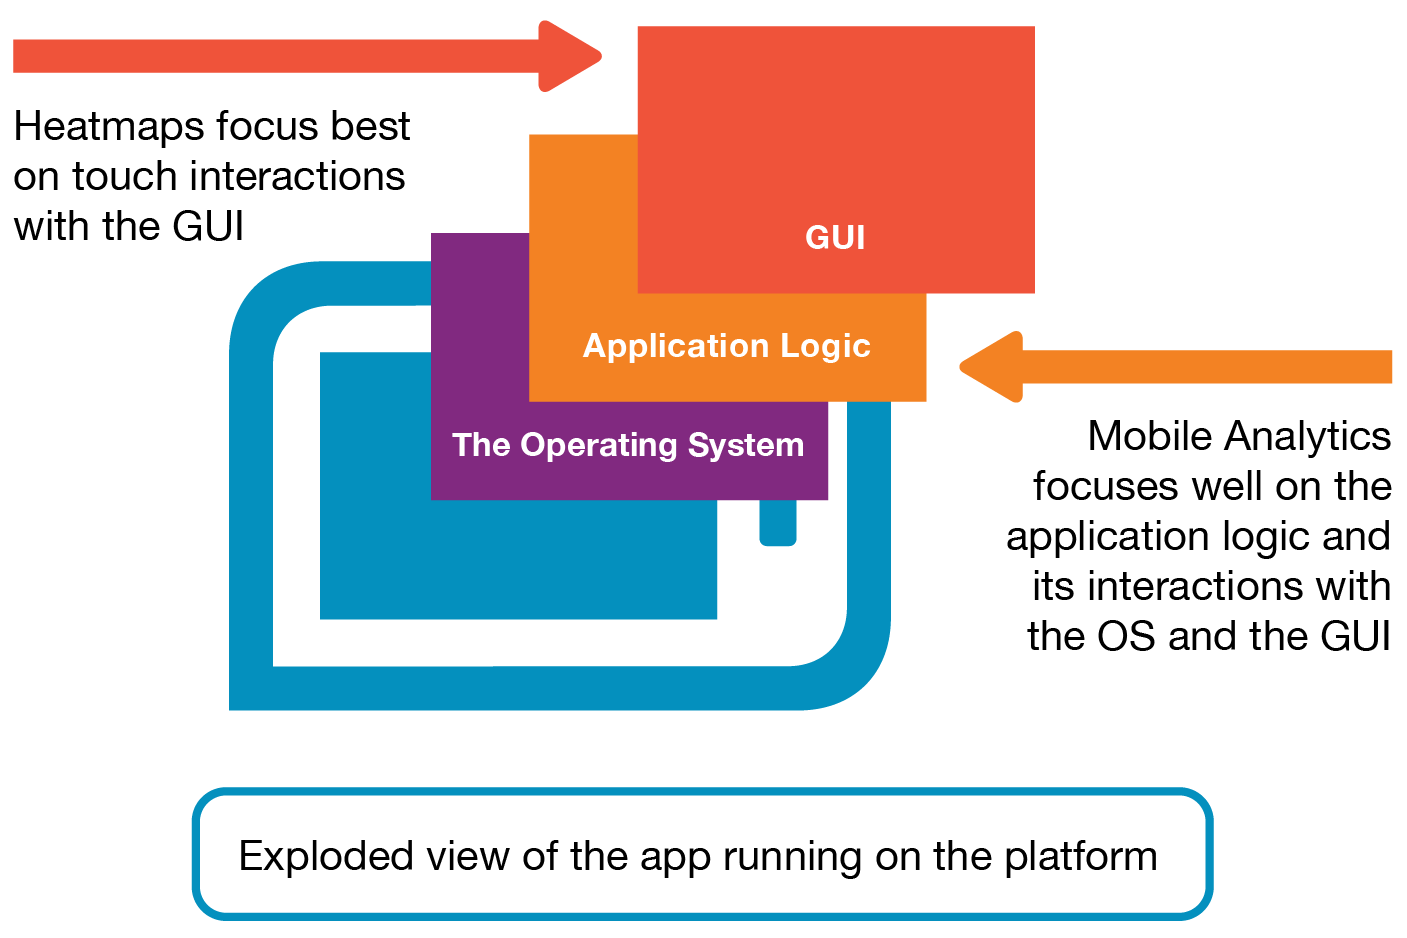
\includegraphics[width=10cm]{images/mobile-analytics-playbook/3-layers.png}
    \caption[Three layers of an app]{Three layers of an app~\footnote{Image credit: First published in the Mobile Analytics Playbook~\cite{harty_aymer_playbook_2016}}.}
    \label{fig:3-layers}
    \end{minipage}
\end{figure}

Of course, apps aren't quite this simple or well defined in reality, for instance they include software libraries from various sources, A/B testing utilities, logging code, run-time lifecycle management, and so on. Nonetheless, these three layers are a useful abstract, particularly in terms of useful observation points about apps on user's computer devices~\footnote{Another observation point that was orthogonal to the application logic layer was one popularised by a company that has since been acquired, called SafeDK. They provided app developers with software that provided an interface between the developer's code and the libraries the code used. This software collected and reported usage data on the performance and reliability of the libraries. Given the commercial nature of the business, their acquisition and the demise of their products and the company's website, and the fast moving nature of the internet, obtaining concrete information may be impractical for all but a few people who know those who were involved at the time.}.

The Graphical User Interface (GUI) % SHOULD-DO add to glossary.
can be visually observed by sighted users, it can also be observed by Accessibility software, and test automation tools, \emph{etc.} externally to the app. It can also be observed from within the app, for instance through using software known as \emph{heatmapping} that records the screens and the touch interactions performed by users of that screen. One of the the more popular, mature heatmapping offerings is from AppSee~\footnote{\url{  https://www.appbrain.com/stats/libraries/details/appsee/appsee}. Note: in 2019 Appsee's team was acqui-hired by ServiceNow~\url{https://techcrunch.com/2019/05/13/servicenow-acquihires-mobile-analytics-startup-appsee/} and the service no longer directly available.}, nonetheless they are only used in a small minority of mobile apps.


\section{Inside-outside perspectives}
As Figure~\ref{fig:internal-external-table} illustrates there are internal and external perspectives on an app for various purposes, including observations, interactions (e.g. through test automation), and emitting information (e.g. through logging, reporting, or mobile analytics). Where the information is observed affects what can be known and what is possible, an insider is privy to information an outsider is not; whereas an outsider has perspective and can potentially perceive things insiders cannot.

\begin{figure}[ht]
    \centering
    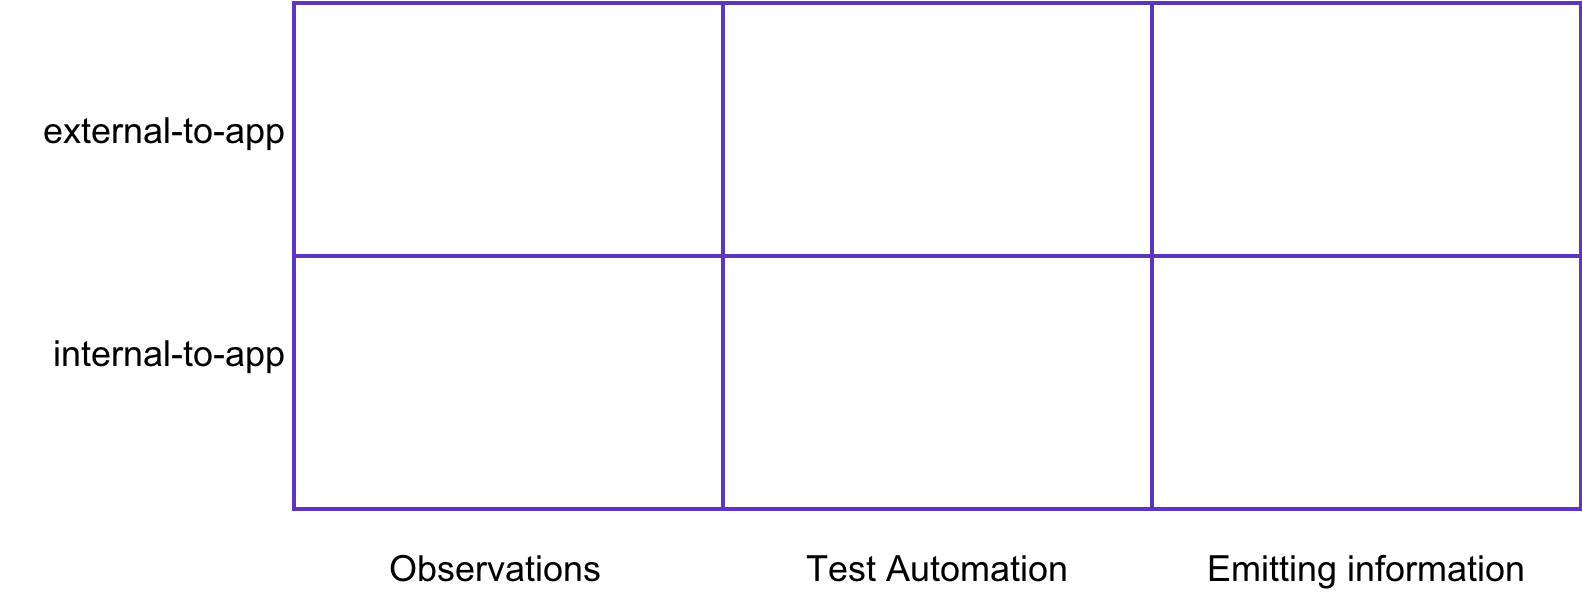
\includegraphics[width=13cm]{images/internal-external-table.png}
    \caption{Internal and external perspectives of an app}
    \label{fig:internal-external-table}
\end{figure}

What is test automation? discuss how mobile apps are tested, the unique aspects of using accessibility interfaces, etc.

\section{Conceptual Model of Usage Analytics}
Conceptually there appear to be four broad levels of usage analytics, these are illustrated in Figure \ref{fig:four-layers-of-analytics-for-mobile-apps} and described next. These four levels can be approximately mapped~\footnote{The approximation is because software is not quite so cleanly cut into layers or levels. For instance app-level mobile analytics can be used to record many aspects of GUI activities, albeit unnaturally. Also, the operating system can observe aspects of the GUI, for instance by instrumenting the Accessibility APIs, a topic I touch on in one of the appendices.} to the three layers of an app:
\begin{itemize}
    \item The Visual [GUI-level] maps to the GUI of the app.
    \item Mobile Analytics maps to the Application layer.
    \item Crashes are considered a liminal level as it can be collected by either or both of the application and the operating system.
    \item Device maps to the operating system of the device.
\end{itemize}
\akb{Don't think you need the list above when you itemise and describe each layer again below}
\akb{Are 'Visual' analytics tools automatically 'Mobile' tools as well? The \textit{heatmapping} example seems to be one that could fit into both layers}

Their use will be discussed in more detail in the chapter titled~\href{chapter-applying-analytics-to-development-practices}{\emph{\nameref{chapter-applying-analytics-to-development-practices}}}. %MUST_DO decide whether layer and level are synonymous, and if not whether to use one term or the other. Anyway I'm aware I may be conflating both terms here and want to improve the precision of whichever term(s) I use. 

\begin{figure}[ht]
    \centering
    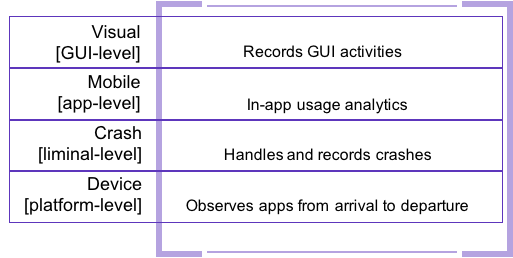
\includegraphics[width=12cm]{images/4-layers-of-analytics.png}
    \caption{Four Layers of Analytics for Mobile Apps}
    \label{fig:four-layers-of-analytics-for-mobile-apps}
\end{figure}

\begin{itemize}
    \item \textbf{Visual (GUI-level)} operates at the GUI level, or layer, of the app. It records aspects of the GUI activities such as touches, gestures, interactions with the screen, and data entry. Often it includes recording what is on the screen too. A common type of Visual analytics is \emph{heatmapping} software.
    \item \textbf{Mobile (app-level)} is incorporated as part of the app and records aspects of what the app is doing, in effect aspects of the usage of the app. Mobile Analytics is prevalent in Android apps and already used for various business purposes.
    \item \textbf{Crash (liminal-level)} is where specialised reporting can intercept crashes. Through the interception they can change the behaviour of the app, for instance to provide a better user-experience, log, and report the crash to the developers. \emph{Fatal crashes} are ones where the application quits. These can also be observed by the operating system; for mobile apps the operating system is an intrinsic part of the platform.
    \item \textbf{Device (platform-level)} Platform-level analytics can record apps from when they are installed until they are removed. This recording can include details such as when apps are in-use, crashes, freezes, and so on. Both of the dominant platforms (iOS and Google Android) allow users to decide whether their devices will share this data.
\end{itemize}

% https://new-wine.org/resources/blog/living-liminality-lessons-trust-gratitude-prayer-compassion-global-church-dd508239ff5

My research includes case studies and developer reports of examples of analytic tools that cover three of these four layers of analytics. The remaining layer, visual analytics, is described briefly with a few examples, visual analytics is seldom used in production mobile apps and therefore I decided to exclude these libraries from my core research. They may be an interesting topic for future research particularly given some of the potential benefits of visual analytics. % COULD_DO add notes on privacy issues and other complicating factors in this sort of research. 


\section{Information sources for app developers}
Developers want and need to know how well their apps are performing from various perspectives such as: growth and adoption (\emph{``do we have more users and are they using the app [more] often?"}), users' ratings and reviews (\emph{``do they like our work?"} and in terms of quality (\emph{``does it perform well? is it fast and reliable?"}). 

\begin{figure}[ht]
    \centering
    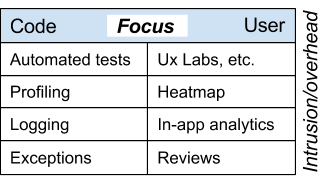
\includegraphics{images/ComparingTechniquesRHS.png}
    \caption{Comparing Techniques}
    \label{fig:comparing_techniques}
\end{figure}

There are various techniques that can be used to assess aspects of quality of mobile apps. Figure \ref{fig:comparing_techniques} provides a visual overview of eight techniques. Of these four are code-oriented and the remaining four more user- or usage- oriented. They are ordered in approximate rank of the overhead, effort, or intrusion involved of each technique. % MUST_DO continue and expand this argument. Discuss why exceptions were chosen as one of the core elements of my research and PhD thesis.

Google's Google Play app store provides developers with answers to all these niggling questions through a developer-oriented user interface called Google Play Console. 
In Google Play Console they provide various tools, reports and data all aimed at informing developers about how their apps are 'doing' and performing. Broadly, these include an overview page with one line of pre-selected data per app managed by the Google Play \textit{Developer Account}. Then, per app, Google provides an overview dashboard of graphs which, in turn, link to more detailed reports and information which provide greater depth. (Examples are provided in the~\href{chapter-analytics-tools}{\emph{\nameref{chapter-analytics-tools}}} chapter.)  Some graphs only appear when Google's algorithms decide they are relevant, these seem to be related to events and/or volumes of underlying data.

\section{Mobile app development lifecycle}
To provide some context for this section, Figure \ref{fig:ci-cd-development-and-feedback}~\footnote{Reproduced from \emph{``An empirical study of architecting for continuous delivery and deployment"}~\cite{shahin2019empirical_study_architecting_cd}}
illustrates a modern continuous software lifecycle including feedback. We can observe several distinct stages in the development and deployment of software and the feedback each stage can provide. %MUST_DO check the guidelines for reproducing and citing a figure as-is.

In contrast, Figure \ref{fig:google-play-app-development-and-feedback} illustrates a similar software lifecycle for Android apps released through Google Play together with the various forms of feedback~\footnote{Here we have excluded feedback from the app store, nonetheless it exists for many app stores.} 

Key differences between typical CI/CD lifecycles and the one for Google Play is the pre-launch testing and the app store providing both user feedback and a service called Android Vitals. The pre-launch reports are generated automatically by Google where the app store runs automated monkey testing on a farm of Android devices and various static analysis checks of releases deployed to any of the test channels. I will explain test channels later on. %MUST_DO actually add information on the test channels and how releases can be promoted to production releases in Google Play.

There are additional sources of \emph{analogue feedback} from people, including from alpha and beta testers and end users; and \emph{digital feedback} from Google tools and from usage data collected from the field. These terms are expanded in the following section~\href{analogue-and-digital-feedback}{\emph{\nameref{analogue-and-digital-feedback}}}.


\begin{figure}[ht]
    \centering
    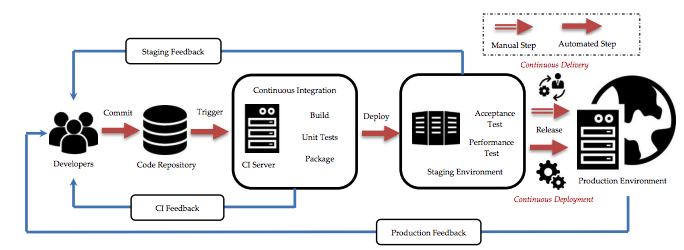
\includegraphics[width=13cm]{images/ci-cd-development-and-feedback.png}
    \caption{CI/CD development and feedback, reproduced from~\cite{shahin2019empirical_study_architecting_cd}}
    \label{fig:ci-cd-development-and-feedback}
\end{figure}

\begin{figure}[ht]
    \centering
    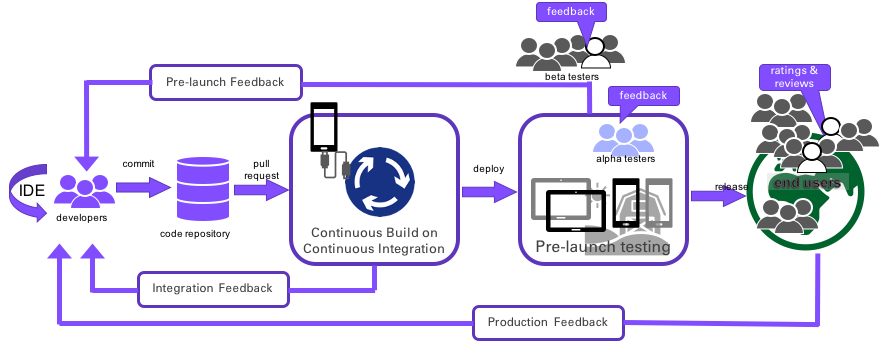
\includegraphics[width=13cm]{images/google-play-app-development.png}
    \caption{Google Play App Development and Feedback}
    \label{fig:google-play-app-development-and-feedback}
\end{figure}


\section{Mobile app usage lifecycle}
Mobile apps have a usage lifecycle, which starts when an app is chosen to be installed and ends with either abandonment or active removal of the app from a device. Figure~\ref{fig:mobile_app_usage_lifecycle}~\footnote{Based on a figure in~\cite{bohmer2011falling_asleep_with_angry_birds}} illustrates the possible stages of a mobile app's life on a user's device. Google Play Console collects data consistent with this lifecycle, analyses it and provides aggregate reports based on their analysis. 

For clarity and completeness there is another lifecycle when the app is running, described in the Android documentation as the \emph{``Processes and Application Lifecycle"}~\cite{android_processes_and_application_lifecycle} These are more detailed and are not included in the reports Google provides (I doubt their details would be recorded either). Note: the processes and application lifecycle may affect how in-app analytics libraries behave, including when they transmit their data to their respective central servers.

% More info and code samples: https://www.vogella.com/tutorials/AndroidLifeCycle/article.html

\begin{figure}[ht]
    \centering
    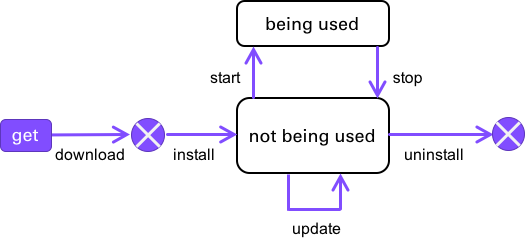
\includegraphics[width=12cm]{images/mobile_app_usage_lifecycle.png}
    \caption{Mobile App Usage Lifecycle}
    \label{fig:mobile_app_usage_lifecycle}
\end{figure}

A later section~\href{platform-level-analytics}{\emph{\nameref{platform-level-analytics}}} provides details of my understanding of how Google collects the underlying data (they do not document, explain or encourage research in how their system works, We return to their behaviour and the effects later in this introduction). And the chapter \href{software-contributions-chapter}{\emph{\nameref{software-contributions-chapter}}} describes software we developed to help collect data from Google Play Console in order to facilitate both research and to enable developers to collect and use data...

Crashes are often considered a concrete measure of poor performance of software and there has been extensive research in crashes for Android applications, in particular. I suspect there are various reasons for the focus on crashes as an oracle for testing software, crashes are unambiguous (even if the causes are not) and they are also binary so easy to determine whether software has, or has not, crashed. 

In 2017, Google launched a service called Android Vitals as a new, intrinsic part of Google Play Console,~\cite{googblogs_I_O_2017_everything_new_in_the_google_play_console}, where they popularised a measure called \emph{Stability} to assess the quality of Android apps. Their measure includes both crashes and when an application freezes or is unresponsive for at least 5 seconds from a user's perspective, a term Google call Application Not Responding (ANR).


\subsection{DevOps}

\begin{figure}
    \centering
    \includesvg[scale=0.8]{images/wikipedia/Yin_yang.svg}
    \caption{Yin Yang to represent DevOps}
    \label{fig:yinyang}
\end{figure}



\section{Analogue and Digital Feedback}~\label{analogue-and-digital-feedback}
Feedback can help developers to find and choose ways to improve their software. Various researchers have investigated way to understand and use feedback provided by end-users, for instance, in ratings and reviews users provide to the app store. For the purposes of my research I term feedback people provide as \emph{analogue feedback} as it has the richness and complexity of analogue signals, and also challenges of processing and comprehension.

In contrast, digital feedback originates from software and is generally deterministic~\footnote{~\url{https://en.wiktionary.org/wiki/deterministic}}. For the purposes of my research I consider digital feedback as that provided by running software where programmers added code to programs to collect data that provides feedback about software use and certain behaviours of that software. The addition of the code may be automated, in part, or wholly, for instance by another program or script. As an example, AppPulse Mobile claims they can add analytics automatically without developers writing a line of code~\footnote{~\url{https://www.microfocus.com/en-us/products/apppulse-mobile-app-apm-monitoring/overview}}.

\subsection{Analogue feedback: in-app tools}

Refer to our Mobile Twin Peaks paper and the concepts, on semi- and structured feedback e.g. surveys, audio recording, etc.

Should I mention app store feedback, probably to provide contrast.


\begin{figure}[ht]
    \centering
    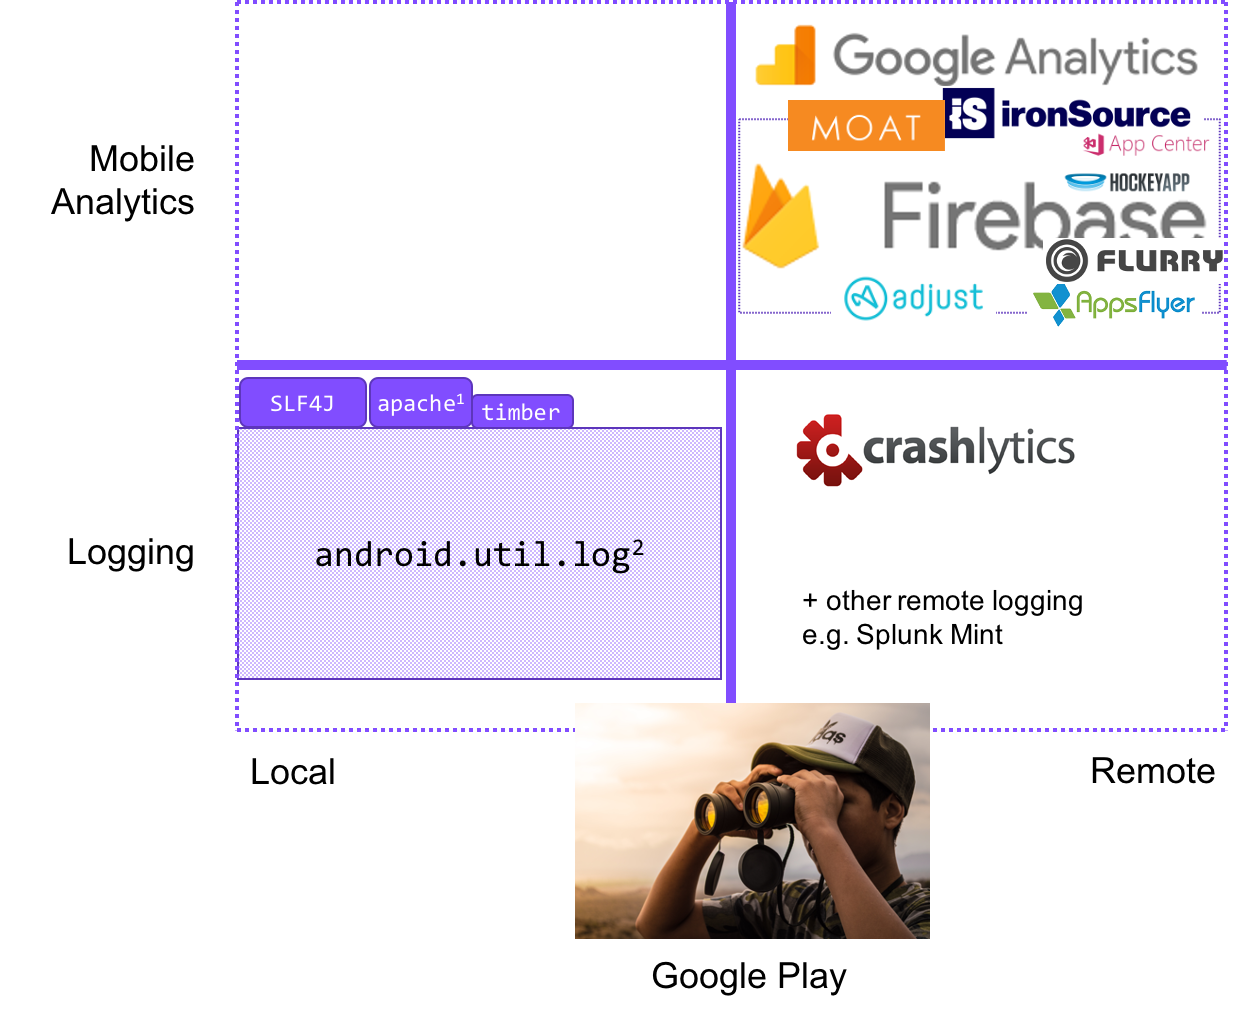
\includegraphics[width=12cm]{images/matrix-of-logging.png}
    \caption{Matrix of logging}
    \label{fig:matrix-of-logging}
\end{figure}

\subsection{Digital feedback: logging and mobile analytics}
The application may incorporate logging and/or mobile analytics. Logging in mobile apps is often used locally, by developers independently of other mechanisms. Figure \ref{fig:matrix-of-logging} illustrates a matrix of logging, where logging and mobile analytics are on the Y axis and local and remote on the X axis. Google Play is an external observer of data recorded in device logs. Data collection runs locally and is sent to Google servers where Google analyses the data and provides reports to developers for their apps.

As an observation the vast majority of Android developers use the default inbuilt logging library \texttt{android.util.log} and choose one or more of Google's analytics offerings (which include Firebase and Crashlytics). A commercial organisation provides current statistics for third-party logging libraries~\footnote{Logging libraries (note the default library is not tracked at the time of writing~\url{https://www.appbrain.com/stats/libraries/tag/logging/logging-libraries}}, crash libraries~\footnote{\url{https://www.appbrain.com/stats/libraries/tag/crash-reporting/android-crash-reporting-libraries}} and mobile analytics~\footnote{\url{https://www.appbrain.com/stats/libraries/tag/analytics/android-analytics-libraries}}. Some apps have several of these libraries so counts may exceed 100\% in their reports.

\begin{itemize}
    \item Logging: enables developers to understand what their software is doing. The practice is commonplace across many software domains including mobile apps, and each platform and language includes a standard method of generating log messages. These messages tend to be small and intended for immediate, local consumption. On Android when developers use the standard logging library (\texttt{android.util.log}) their log messages are written to a shared circular log file on a device. Some privileged Android software is able to read these shared logs, developers can also read them using standard Android development tools \emph{e.g.} \texttt{adb logcat} providing they are connected to the device with the log file. Older versions of Android allowed apps to read the full contents, more recently apps are restricted to only the log messages they wrote unless they are granted the relevant permission by Google and the user. 
    In other domains \emph{e.g.} web servers, infrastructure software, and many others, logging is used for production monitoring, fault-finding and analysis. A minority of mobile app developers use remote logging.
    \item Mobile analytics, can extend and scale logging. For mobile analytics, a minority of developers incorporate custom implementations, however the vast majority who use analytics do so through using third-party analytics libraries such as Google Firebase Analytics, details of the current usage of analytics libraries are provided by AppBrain~\footnote{\url{https://www.appbrain.com/stats/libraries/tag/analytics/android-analytics-libraries}}.
\end{itemize}

\subsection{Designing the content/messages} 
% I'm not sure whether content or messages, or a mix of both words, best encompasses the topic I wish to discuss here. Messages can have content, however sometimes a message is a message by its existence, even with no payload. (2 rings on the home phone when you arrive, told the family you'd arrived without needing to pay for the telephone call. Heartbeat messages in systems, etc.). Also the design may include non-content aspects, content transformations, etc. Anyway, let's get writing. 
This section applies to messages that an app could emit regardless of the conduit (\emph{i.e.} it applies to logging and using mobile analytics). At the risk of some ambiguity, the term log will be used to reflect both logging and mobile analytics in this section to improve overall readability.

\emph{Related concepts}: The uneven U, computer protocols (layers, formatting, and contents), structured messages, what to log. %MUST_DO expand this section.

There are many choices that can be considered in terms of designing the content/messages. For various reasons developers may pay little strategic attention to logging in their daily work. For those who do choose to consider logging strategically there are various considerations, including:
What to log, how to log, where to log, data transformations, delivery mechanisms and characteristics.

Developers have control over what to log, how, and when to generate the log messages. They may be constrained in various ways by APIs, message lengths, encoding, and formats, access to messages, and when messages will be transmitted, \emph{etc.} 

It is possible to test the constraints, for instance by writing custom automated tests and/or apps that generate a variety of messages where the outputs are checked somehow. The checking may be partly or completely performed programmatically (we did some unpublished research in this area in 2018).

The purpose of the message may differ in the type and level of information it is intended to convey. Some messages may contain low-level, or detailed, error messages intended to help improve the technical aspects of the software to make the software more robust. Other messages may aim to communicate intent, completion of a task, activity or user-journey in the software. For example, IBM published a paper about software called CX Mobile that aims to record and visualise user journeys for iOS and Android apps~\cite{hu_tealeaf_cxmobile}.


The distinction between analytics and logging may be murky. A pragmatic heuristic is to use the declared category of the library, tool or service, for instance Firebase analytics would be considered as analytics whereas Timber.io would be considered as logging even though both contain aspects of the other category.

Similar to the concept of black box testing (where software's behaviour is observed and assessed without knowing the internals), external software can observe the behaviours of apps. Google have developed and integrated software that monitors apps running in Google approved versions of Android. The data is collected per device and provided automatically to Google servers if the device has the relevant settings enabled~\cite{google_play_share_usage_and_diagnostics_info_with_google}. This data is processed by Google who provide some portions of the data to the registered developers of that app in the Google Play Store.

\emph{Idea for expansion:} Drop-off in data for a population  c.f. marketing funnels, funnels for shopping carts, etc.

% Mobile Developer's Guide to the fifth dimension
% available from https://www.dropbox.com/s/no70z2hiod6z7o8/Fifth_Dimension_v1.pdf?dl=0 (took 20 - 30 mins to track down)

\subsection{The mechanics of sending data}
To be useful the analytics data needs to reach the system that processes, analyses and reports on it. There are various mechanisms that can be used to send data ranging from unlikely (at least for the app store ecosystems and their apps), retyping, transferring using USB devices, etc. to the most likely which uses a valid internet connection over WiFi or a mobile network. 

MUST-DO expand the following lists.
\begin{itemize}
    \item Triggers, batching, caps/buffers/limits, availability of any connection, or only approved connection, priorities, latency, delays,
    \item Permissions (including permissions to access the source data on the device and permission to share it (and permission to use certain connections/times/etc.)
    \item authorisation and authentication, spoofing and poisoning,
    \item freshness|staleness of the data, encoding, ...
    \item Lean data, privacy and sensitivity of the contents, data quality, encoding, ...
    \item Screening and filtering: who, when, how, why.
\end{itemize}

Examples:
\begin{itemize}
    \item Fabric Crashlytics, batching and caps/limits.
    \item Mozilla Glean telemetry.
\end{itemize}



\section{Passive, tacit, and explicit analytics choices}
Various degrees of choices are available depending on how actively the development team wishes to incorporate analytics into their development practices. These include using what already exists, where the data is gathered by others and made available to the developers, here these sources are called \emph{passive analytics}. Developers can choose to take more authority in the data collection, for instance by deciding what data they would like to collect and how they wish to collect it. They can use these tools at various depths, ranging from superficial use to actively maximising the efficacy of using analytics to provide them with the data they believe they need to achieve their outcomes. There is an interesting discussion in a blog article~\cite{mukherjee_implicit_versus_explicit_event_tracking_hits_and_misses} on what they term \emph{implicit, or codeless} and \emph{explicit or code-based} event tracking using web analytics tools. The article compares the benefits (hits) and flaws (misses) of both approaches. It also provides a flow chart to help teams select analytics tools that suit their context.

% More reading
% https://web.archive.org/web/20120401053907/http://www.wiikno.com/blog/explicit-vs-implicit-data


\subsection{Passive Analytics}~\label{subsection-passive-analytics}
Passive analytics are those not actively under the control or influence of the development team, they are provided from other sources such as the operating system or the app store. In my research the passive analytics are all managed by the app store, Google Play Console.

\subsection{Tacit Analytics}~\label{subsection-tacit-analytics}
Tacit is variously defined as \emph{``Something tacit is implied or understood without question."}~\footnote{\url{https://www.vocabulary.com/dictionary/tacit}}, \emph{``Understood or implied without being stated."}~\footnote{\url{https://www.lexico.com/en/definition/tacit}, Note: Lexico.com is a new collaboration between Dictionary.com and Oxford University Press~\url{https://www.lexico.com/about}}, silent, wordless, or noiseless. 
%
It may be something that is inherent in the nature of using many of the third-party analytics libraries. In my research I consider tacit analytics to be that where developers accept whatever default data is collected by an analytics library without the developer needing to do anything more than integrate the library into their app. 

\subsection{Explicit Analytics}~\label{subsection-explicit-analytics}
Explicit analytics is where developers have actively added code to interact with analytics libraries, for instance by calling methods in the API(s) provided by the library's. There are various degrees of use of the APIs and developers may have various intentions for calling these APIs.


\section{Summary of the background chapter}
This chapter has introduced various concepts and topics which help provide context for the rest of this thesis. Some additional background material is available in various appendices, including more information on mobile analytics and various software contributions.
